%%%%%%%%%%%%%%%%%%%%%%%%%%%%%%%%%%%%%%%%%%%%%%%%%%%%%%%%%%%%%%%%%%%%%%%%%%%%
% AGUJournalTemplate.tex: this template file is for articles formatted with LaTeX
%
% This file includes commands and instructions
% given in the order necessary to produce a final output that will
% satisfy AGU requirements, including customized APA reference formatting.
%
% You may copy this file and give it your
% article name, and enter your text.
%
%
% Step 1: Set the \documentclass
%
%

%% To submit your paper:
\documentclass[draft]{agujournal2019}
\usepackage{url} %this package should fix any errors with URLs in refs.
\usepackage{lineno}
\usepackage[inline]{trackchanges} %for better track changes. finalnew option will compile document with changes incorporated.
\usepackage{soul}
\usepackage{float}
\usepackage[T1]{fontenc}
\linenumbers
%%%%%%%
% As of 2018 we recommend use of the TrackChanges package to mark revisions.
% The trackchanges package adds five new LaTeX commands:
%
%  \note[editor]{The note}
%  \annote[editor]{Text to annotate}{The note}
%  \add[editor]{Text to add}
%  \remove[editor]{Text to remove}
%  \change[editor]{Text to remove}{Text to add}
%
% complete documentation is here: http://trackchanges.sourceforge.net/
%%%%%%%

\draftfalse

%% Enter journal name below.
%% Choose from this list of Journals:
%
% JGR: Atmospheres
% JGR: Biogeosciences
% JGR: Earth Surface
% JGR: Oceans
% JGR: Planets
% JGR: Solid Earth
% JGR: Space Physics
% Global Biogeochemical Cycles
% Geophysical Research Letters
% Paleoceanography and Paleoclimatology
% Radio Science
% Reviews of Geophysics
% Tectonics
% Space Weather
% Water Resources Research
% Geochemistry, Geophysics, Geosystems
% Journal of Advances in Modeling Earth Systems (JAMES)
% Earth's Future
% Earth and Space Science
% Geohealth
%
% ie, \journalname{Water Resources Research}

\journalname{Geophysical Research Letters}


\begin{document}

%% ------------------------------------------------------------------------ %%
%  Title
%
% (A title should be specific, informative, and brief. Use
% abbreviations only if they are defined in the abstract. Titles that
% start with general keywords then specific terms are optimized in
% searches)
%
%% ------------------------------------------------------------------------ %%



\title{The contribution of drifting snow to cloud properties and the atmospheric radiative budget over Antarctica}

%% ------------------------------------------------------------------------ %%
%
%  AUTHORS AND AFFILIATIONS
%
%% ------------------------------------------------------------------------ %%

% Authors are individuals who have significantly contributed to the
% research and preparation of the article. Group authors are allowed, if
% each author in the group is separately identified in an appendix.)

% List authors by first name or initial followed by last name and
% separated by commas. Use \affil{} to number affiliations, and
% \thanks{} for author notes.
% Additional author notes should be indicated with \thanks{} (for
% example, for current addresses).

% Example: \authors{A. B. Author\affil{1}\thanks{Current address, Antartica}, B. C. Author\affil{2,3}, and D. E.
% Author\affil{3,4}\thanks{Also funded by Monsanto.}}

\authors{Stefan Hofer\affil{1}, Charles Amory\affil{2,3}, Christoph Kittel\affil{2}, Tim Carlsen\affil{1}, Louis Le Toumelin\affil{4}\,and Trude Storelvmo\affil{1}}


% \affiliation{1}{First Affiliation}
% \affiliation{2}{Second Affiliation}
% \affiliation{3}{Third Affiliation}
% \affiliation{4}{Fourth Affiliation}

\affiliation{1}{Department of Geosciences, University of Oslo, Oslo, Norway}
\affiliation{2}{Department of Geography, SPHERES Research Unit, University of Liège, Liège, Belgium}
\affiliation{3}{Univ. Grenoble Alpes, CNRS, Institut des Géosciences de l’Environnement, Grenoble, France}
\affiliation{4}{Univ. Grenoble Alpes, Université de Toulouse, Météo-France, CNRS, CNRM, Centre d’Études de la Neige, Grenoble, France}
%(repeat as many times as is necessary)

%% Corresponding Author:
% Corresponding author mailing address and e-mail address:

% (include name and email addresses of the corresponding author.  More
% than one corresponding author is allowed in this LaTeX file and for
% publication; but only one corresponding author is allowed in our
% editorial system.)

% Example: \correspondingauthor{First and Last Name}{email@address.edu}

\correspondingauthor{Stefan Hofer}{stefan.hofer@geo.uio.no}

%% Keypoints, final entry on title page.

%  List up to three key points (at least one is required)
%  Key Points summarize the main points and conclusions of the article
%  Each must be 100 characters or less with no special characters or punctuation and must be complete sentences

% Example:
% \begin{keypoints}
% \item	List up to three key points (at least one is required)
% \item	Key Points summarize the main points and conclusions of the article
% \item	Each must be 100 characters or less with no special characters or punctuation and must be complete sentences
% \end{keypoints}

\begin{keypoints}
\item Accounting for drifting snow over Antarctica leads to a radiative forcing of +2.7\,Wm\textsuperscript{-2} over the grounded ice sheet
\item Accounting for drifting snow increases the cloud cover over Antarctica by 18.6\%
\item Drifting snow is an important - yet in climate models and observations often neglected - component of the Antarctic surface energy budget
\end{keypoints}

%% ------------------------------------------------------------------------ %%
%
%  ABSTRACT and PLAIN LANGUAGE SUMMARY
%
% A good Abstract will begin with a short description of the problem
% being addressed, briefly describe the new data or analyses, then
% briefly states the main conclusion(s) and how they are supported and
% uncertainties.

% The Plain Language Summary should be written for a broad audience,
% including journalists and the science-interested public, that will not have 
% a background in your field.
%
% A Plain Language Summary is required in GRL, JGR: Planets, JGR: Biogeosciences,
% JGR: Oceans, G-Cubed, Reviews of Geophysics, and JAMES.
% see http://sharingscience.agu.org/creating-plain-language-summary/)
%
%% ------------------------------------------------------------------------ %%

%% \begin{abstract} starts the second page

\begin{abstract}
The Antarctic Ice Sheet experiences perpetual katabatic winds, transporting snow and moisture from the interior towards the periphery. However, the impacts of Antarctic moisture and drifting snow on cloud structure and surface energy fluxes have not been widely investigated. Here, we use a regional climate model with a newly-developed drifting snow scheme to show that accounting for drifting snow notably alters the spatial distribution, vertical structure and radiative effect of clouds over Antarctica. Overall, we find that accounting for drifting snow leads to a greater cloud cover providing an increase of +2.74\,Wm\textsuperscript{-2} in the surface radiative energy budget. Additionally, a comparison with 20 weather stations reveals a 2.17\,Wm\textsuperscript{-2} improvement in representing the radiative energy fluxes. Our results highlight the need to study the impact of missing drifting snow processes on the future evolution of clouds, the surface energy budget and the vertical atmospheric structure over Antarctica.
\end{abstract}

\section*{Plain Language Summary}
Antarctica is the continent with the strongest winds on Earth. These winds pick up a lot of snow on their way from the interior towards the ocean, forming drifting snow clouds. Drifting snow clouds can extend over 1000 km horizontally and multiple 100 m vertically. Like a normal cloud, they can reflect incoming sunlight like a mirror and trap heat like a blanket. However, most of our climate models don't yet incorporate these drifting snow clouds and therefore might be missing an important part of the Antarctic climate system. In this study we show that when we account for drifting snow clouds the Antarctic surface receives notably more thermal radiation. Additionally, we also show that we significantly improve our model when we include blowing snow by comparing our outputs to weather station observations over Antarctica. Therefore, we conclude that accurate sea level rise projections need to account for drifting snow.


%% ------------------------------------------------------------------------ %%
%
%  TEXT
%
%% ------------------------------------------------------------------------ %%

%%% Suggested section heads:
% \section{Introduction}
%
% The main text should start with an introduction. Except for short
% manuscripts (such as comments and replies), the text should be divided
% into sections, each with its own heading.

% Headings should be sentence fragments and do not begin with a
% lowercase letter or number. Examples of good headings are:

% \section{Materials and Methods}
% Here is text on Materials and Methods.
%
% \subsection{A descriptive heading about methods}
% More about Methods.
%
% \section{Data} (Or section title might be a descriptive heading about data)
%
% \section{Results} (Or section title might be a descriptive heading about the
% results)
%
% \section{Conclusions}


\section{Introduction}
Due to strong surface radiative cooling in the interior Antarctic plateau, strong and perpetual katabatic winds emerge \cite{Parish2007}, redistributing snow mass from the interior of Antarctica towards the edges and ice shelves \cite{Lenaerts2012b}, where the roughly 4~km high plateau slopes steeply towards sea level. These perpetual katabatic winds pick up snow from the ground once they reach a threshold wind speed and create a drifting-snow cloud \cite{Schmidt1980,Amory2017}. These drifting-snow clouds can extend over several 100\,m in the vertical direction \cite{Mann2000, Gossart2017, Mahesh2003}, and multiple 100\,km in the horizontal \cite{Palm2018, Mahesh2003, Yang2021}.

Clouds are known to notably affect the present and future climates of polar ice sheets \cite{Gilbert2020,Gorodetskaya2015,Lachlan2010,Hofer2017, Hofer2019,Hahn2019}. They have the ability to amend incoming and outgoing shortwave and longwave fluxes, depending on the cloud phase, height and particle size distribution, directly impacting the surface energy budget \cite{Gilbert2020,Tan2016,Tan2019}. Optically-thick drifting-snow clouds, while not accounted for in most global and regional climate models, can change the atmospheric radiation budget \cite{Letoumelin2020}, most notably because drifting-snow layers act as a cloud themselves, increasing the atmospheric longwave emissivity and decreasing the shortwave transparency of the atmosphere \cite{Yang2013, Yamanouchi1984, Letoumelin2020, Lawson2006}. Further, drifting-snow sublimation acts as a moisture source and a heat sink and therefore changes the temperature and humidity distribution in the near-surface atmosphere \cite{Amory2019}. Additionally, drifting-snow particles can also act as ice nucleating particles for cloud formation \cite{Geerts2015}, which impact the longevity, structure, cloud-phase distribution and precipitation formation within pre-existing clouds. While the near-surface air temperatures in the interior of Antarctica are often below -37\,\textdegree C, where homogenous cloud droplet freezing glaciates all clouds, above the boundary layer mixed-phase clouds can still exist in the Antarctic interior \cite{Lawson2014}, which are susceptible to changes in available ice nuclei. However, so far very little is known about how clouds are influenced by drifting-snow processes in climate models, and how accounting for drifting snow over the current climate influences key polar cloud-, and therefore climate processes.

Here, we use two regional climate model simulations spanning the period of 2000-2019, one with a dynamic representation of drifting snow and one without, to assess the impact of accounting for drifting snow on the representation of Antarctic clouds and surface radiative fluxes. We compare our two simulations during the 2000-2019 period to concurrently available satellite products of cloud cover and the ERA5 reanalysis, to show whether accounting for drifting snow only amends or also improves the comparison of modelled to observed Antarctic clouds. However, current satellite cloud cover products over Antarctica often do not report values in the lowermost 100 m  of the atmosphere where drifting snow is frequent and therefore neglect drifting snow and render model cloud cover verification difficult. Nevertheless, our results deliver a clear indication that accounting for drifting snow over polar ice sheets changes the 3D-structure of clouds and ultimately their contribution to the surface energy budget. Due to their similarity in radiative effects and also particle size \cite{Lawson2006}, we think that thick drifting-snow layers should be referred to as drifting-snow clouds and be included in satellite products used for model cloud cover evaluation. In conclusion, not accounting for drifting snow in future projections of the Antarctic climate and sea level rise contribution might significantly bias the drawn conclusions.

\section{Materials and Methods}

\subsection{MAR}
We use simulations performed with MAR \cite{Fettweis2013a, Hofer2020}, a hydrostatic, polar-oriented, regional climate model extensively evaluated over Antarctica \cite{Agosta2019, Mottram2020, Kittel2021} . The microphysical scheme of MAR solves conservation equations for five atmospheric water species including specific humidity, cloud droplets, rain drops, cloud ice crystals, and snow particles \cite{Gallee1994}. Radiative transfer in the atmosphere is adapted from \citeA{Morcrette2002}. Energy and mass transfer between the atmosphere and the snow/ice surface are achieved through the coupling of MAR with the one-dimensional surface scheme SISVAT (Soil Ice Snow Vegetation Atmosphere Transfer) \cite{DeRidder1998, Gallee1997, Gallee2001}, which includes a detailed representation of snow/firn/ice properties inspired from an early version of the CROCUS snow model \cite{Brun1992}.

In this study, we used the latest model version of MAR (v3.11), which includes a recently updated drifting-snow scheme described and evaluated in \citeA{amory2021}. Erosion of snow in the model occurs when the wind shear stress exerted at the surface exceeds a threshold value that depends only upon surface snow density ($\rho_{s}$) when $\rho_{s}$ < 450 kg/m\textsuperscript{3}.

Once removed from the surface, eroded particles are mixed with the pre-existing windborne snow mass and their interactions with the atmosphere are computed by the microphysical and the radiative transfer schemes. In particular, the latent heat uptake and moisture release due to sublimation of suspended snow particles is accounted for in the energy and mass budget of each atmospheric level in which sublimation occurs, and suspended snow particles are included in the computation of cloud radiative properties \cite{Gallee2010}. 

In both simulations, in which drifting snow was respectively switched on and off, we prescribed lateral, top-of-atmosphere and sea surface conditions from 6-hourly ERA5 reanalysis \cite{Hersbach2020}. We ran MAR at a spatial resolution of 35 km x 35 km and used 24 vertical levels to describe the atmosphere, with a higher vertical resolution in the low troposphere and a lowest level situated at 2 m above ground level.

For the comparison with in situ radiative observations, model results for surface radiative fluxes are extracted from the 4 closest grid cells to the observation location following the same method described in \citeA{Mottram2020} for the comparison with weather observations.

\subsection{CloudSat-CALIPSO cloud fraction}
For the comparison of the cloud cover simulated by MAR with satellite observations, we use the combined CloudSat spaceborne radar and CALIPSO spaceborne lidar cloud fraction dataset \cite{kay2009}. It is based on the R04 versions of the CloudSat standard products 2B-GEOPROF \cite{marchand2008} and 2B-GEOPROF-LIDAR \cite{mace2009} and provides the cloud fraction globally (82°S-82°N) on a 2°\,x\,2° horizontal grid with a 480\,m vertical resolution. The great advantage of using this active remote sensing dataset is its independence from the surface albedo over the bright Antarctic \cite{kay2016}. Here, we use the total mean cloud fraction between July 2006 and February 2011. Note however, that the widely-used CloudSat-CALIPSO cloud fraction product ignores cloud cover below 720 m, the part of the atmosphere where drifting-snow clouds are most frequently observed.

\section{Results}

\subsection{Influence of drifting snow on the vertical atmospheric structure}

Explicitly modelling drifting snow in MAR leads to a notable change in the atmospheric structure of the lowermost 100s of meters above ground (Fig.\ref{fig:Test} A-C). Over the flat interior of the Antarctic Ice Sheet, the first few 100\,m show a strong decrease in atmospheric temperature, with a mean 0-500\,m difference of -0.66 $\pm$ 0.40\,\textdegree C in elevations greater than 2000\,m above mean sea level (Fig.\ref{fig:Test} A). Conversely, over the lower grounded ice and the low-lying ice shelves surrounding the Antarctic Ice Sheet (<100\,m above sea level), this decrease in temperature in the drifting snow simulations is less notable. The mean 0-500\,m above surface difference lies at -0.23 $\pm$ 0.15\,\textdegree C. The contrasting picture between the flat interior and the steeper and lower margins of Antarctica is likely caused by a contrast in atmospheric turbulence: 1) Due to the low height gradients over the interior plateau and the corresponding stable boundary layer and less pronounced effect of turbulent mixing, the sublimational cooling is not mixed as efficiently as over the steeper margins. Therefore, we see a stronger boundary layer cooling in the interior when accounting for drifting snow sublimation, despite lower total erosion of snow by the wind than over steeper terrain. Sublimation cools the atmosphere because the change of water phase from solid to gaseous requires energy from the surrounding air to break up the bonds between the H$_2$O molecules, leading to a drop in temperature. 2) Due to adiabatic warming and strong turbulent mixing in areas where the gravitational pull accelerates the katabatic winds down steep terrain, the height of the boundary layer increases and the particles are entrained into higher elevations. Therefore, the sublimational cooling is less concentrated over the margins of Antarctica and the ice shelves, despite a greater sublimation potential due to higher temperatures and increased erosion fluxes over the steeper margins.

\begin{figure}[H]
	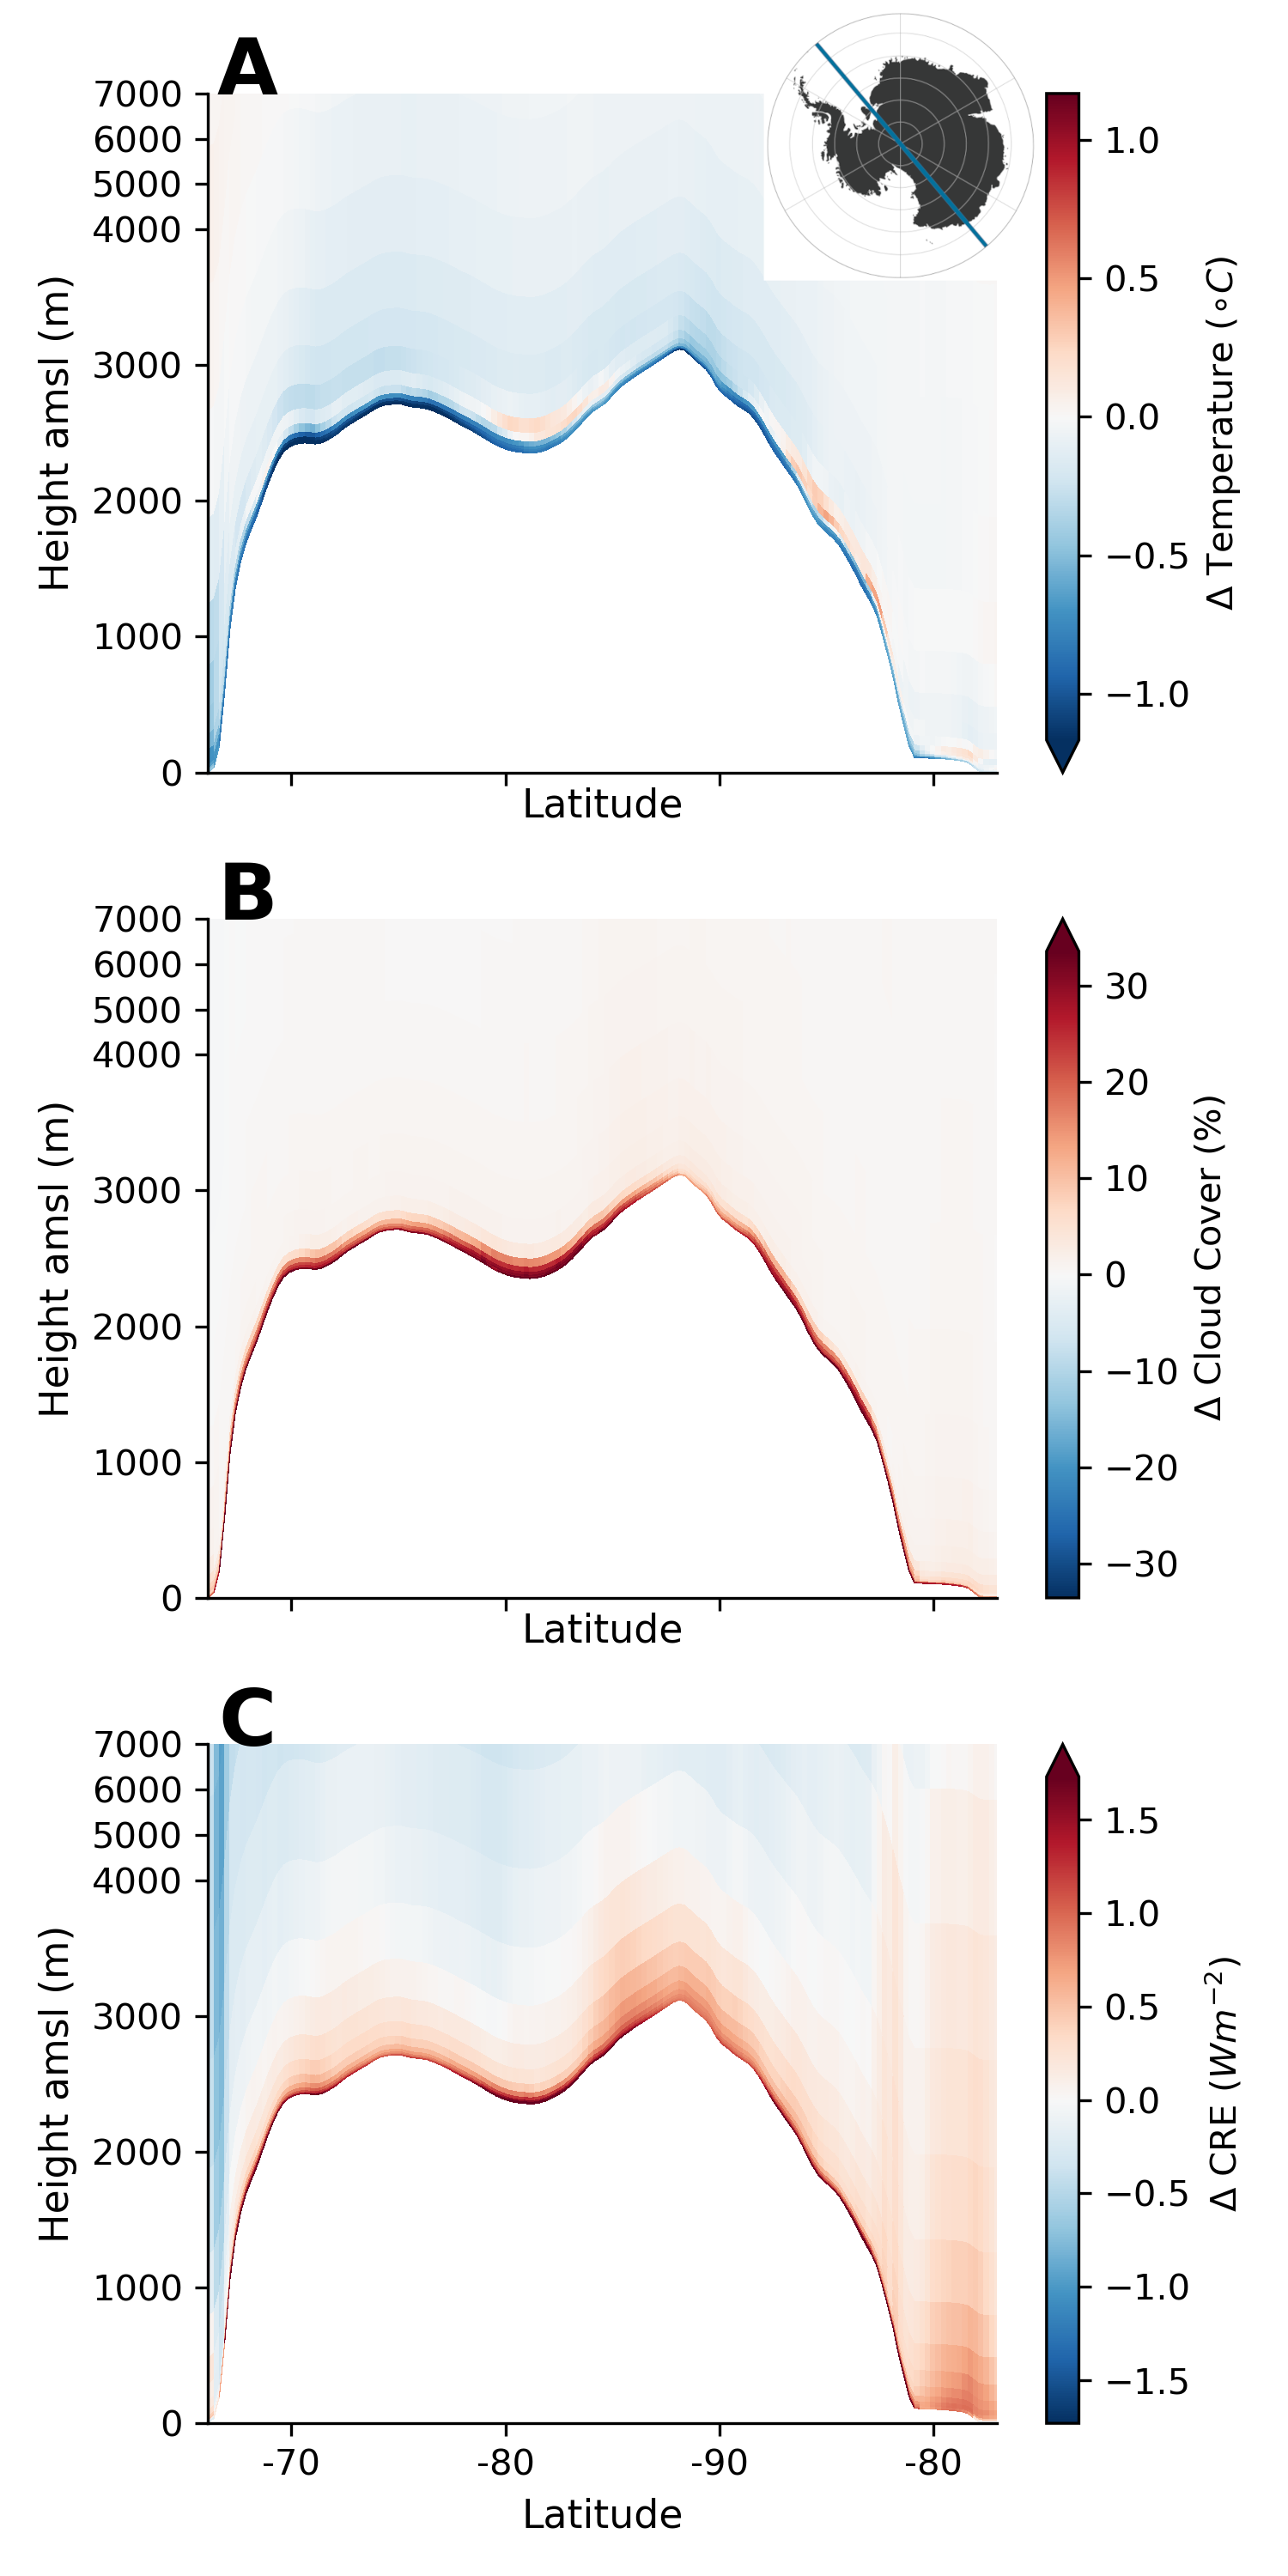
\includegraphics[width=0.5\textwidth]{cross_section_lt_new.png}
	\caption{\textbf{Difference in temperature and cloud properties between MAR with and without drifting snow during 2000-2019.} A) Cross-section of temperature differences between MAR with drifting snow turned on, and MAR without drifting snow (positive means MAR with drifting snow is warmer), along the path shown in the inset at the top right of the panel. B) Same as panel A), but showing the difference in cloud cover (in \%) between the two simulations. C) Same as panel A) and B), but for the difference in the cloud radiative effect ($Wm^{-2}$). }
	\label{fig:Test}
\end{figure}

In the boundary layer, accounting for drifting snow also increases cloud ocurence over the Antarctic continent (Fig.\ref{fig:Test}B). Our results show that the strongest increase in 2000-2019 average cloud cover over the interior plateau strongly overlap with the changes in temperature seen in Figure \ref{fig:Test}A. In elevations above 2000\,m above mean sea level the lowermost 500\,m of the atmosphere show an increase of +18.4 $\pm$ 11.8\% in cloud cover. Again, over lower elevations (<100 m) the signal is less pronounced, with an increase in cloud cover of +12.5 $\pm$ 8.4\%.

Generally, there are three overlapping mechanisms that can explain the greater cloud amount over Antarctica, when accounting for drifting snow. 1) Thick drifting-snow layers themselves act as a cloud, due to their ability to interact with incoming solar radiation (i.e. a cloud optical depth > 0) and their influence on the atmospheric longwave emissivity (i.e. they increase the atmospheric longwave emissivity $\epsilon$). 2) The sublimation of airborne snow particles leads to a cooling of the surrounding air, while increasing the specific humidity, both bringing the environment closer to saturation \cite{Amory2019}. 3) Drifting snow particles can act as additional nuclei on which water vapor can sublimate or help with ice growth through the Wegener-Bergeron-Findeisen process in mixed-phase clouds above the boundary layer. Ice crystal number concentration can furthermore potentially multiply through secondary ice processes \cite{Soti2020}. It is likely that in most cases these three processes can act simultaneously. 

Accounting for drifting snow also alters the cloud radiative effect, defined here as the difference between the net radiative fluxes in all-sky conditions and under clear-sky conditions ($CRE= N_{all-sky} - N_{clear-sky}$, where N is the net radiation at the surface, Fig.\ref{fig:Test} C). Again, we see the most notable changes in the boundary layer over the interior plateau of Antarctica. In areas above 2000\,m above mean sea level, the CRE increases by +1.0 $\pm$ 0.5\,Wm\textsuperscript{-2} in the lowermost 500\,m of the atmosphere. Conversely, the changes in the cloud radiative effect are virtually negligible over the margins and ice shelves with +0.1 $\pm$ 0.3\,Wm\textsuperscript{-2}.

While we see the strongest effects again in the boundary layer of the interior plateau, especially over the steeper margins, the CRE is altered up to elevations of roughly 5000\,m above ground. This vertical influence on the CRE might be due to the fact that drifting-snow particles can be mixed to layers above the boundary layer in zones with stronger adiabatic mixing and turbulence, i.e. over the steeper slopes where the katabatic winds are the strongest. Subsequently, these additional solid particles (i.e, snow and ice crystals) can influence the macrophysical cloud properties in our model (ice water path, liquid water path and cloud optical depth), and therefore the cloud radiative effect. Additionally, because of changes in the vertical temperature distribution and humidity due to drifting-snow sublimation, also the emissivity and temperature of the layers that emit the longwave radiation can be altered between the two simulations.

\subsection{Influence of drifting snow on cloud properties}

%Differences over various areas
%LWP: Grounded=0.01, Shelves=0.05, Ocean=-0.02
%IWP: Grounded=5.44, Shelves=8.59, Ocean=2.86
%COD: Grounded=0.00, Shelves=0.00, Ocean=-0.02
%CC: Grounded=17.61, Shelves=13.96, Ocean=9.93
%For comparison
%Means over shelf+ground: COD=0.01, IWP=61.55, LWP=0.17
%Means over ground: COD=0.01, IWP=56.74, LWP=0.14
%Means over shelves: COD=0.03, IWP=111.04, LWP=0.54

%With updated files (no 5% RH increase)
%LWP: Grounded=0.01, Shelves=0.05, Ocean=nan
%IWP: Grounded=5.90, Shelves=9.09, Ocean=nan
%COD: Grounded=0.00, Shelves=0.00, Ocean=nan
%CC: Grounded=18.64, Shelves=14.54, Ocean=nan
%Means over shelf+ground: COD=0.01, IWP=62.21, LWP=0.17
%Means over ground: COD=0.01, IWP=57.40, LWP=0.14
%Means over shelves: COD=0.03, IWP=111.68, LWP=0.54

To explore how the macrophysical cloud properties in MAR with drifting snow differ from the control simulation without drifting snow, we show the spatial difference in cloud cover, cloud optical depth, liquid- and ice water path in Fig.\ref{fig:micro} A-D.

Overall, our results show a clear signal of increased cloud cover over most of Antarctica. Over the grounded ice sheet the increase in cloud cover is most notable with +18.6\,\%, but it also increases strongly over the low-lying ice shelves (+14.5\,\%). Over most of Antarctica our results indicate no changes in mean annual cloud optical depth (Fig.\ref{fig:micro}B), however over Antarctica most of the year solar radiation is absent. Interestingly, around the Antarctic peninsula we see areas with a slightly more notable COD increase of up to +0.03, which is of the same order of magnitude as the mean cloud optical depth over all the ice shelves.

\begin{figure}[H]
	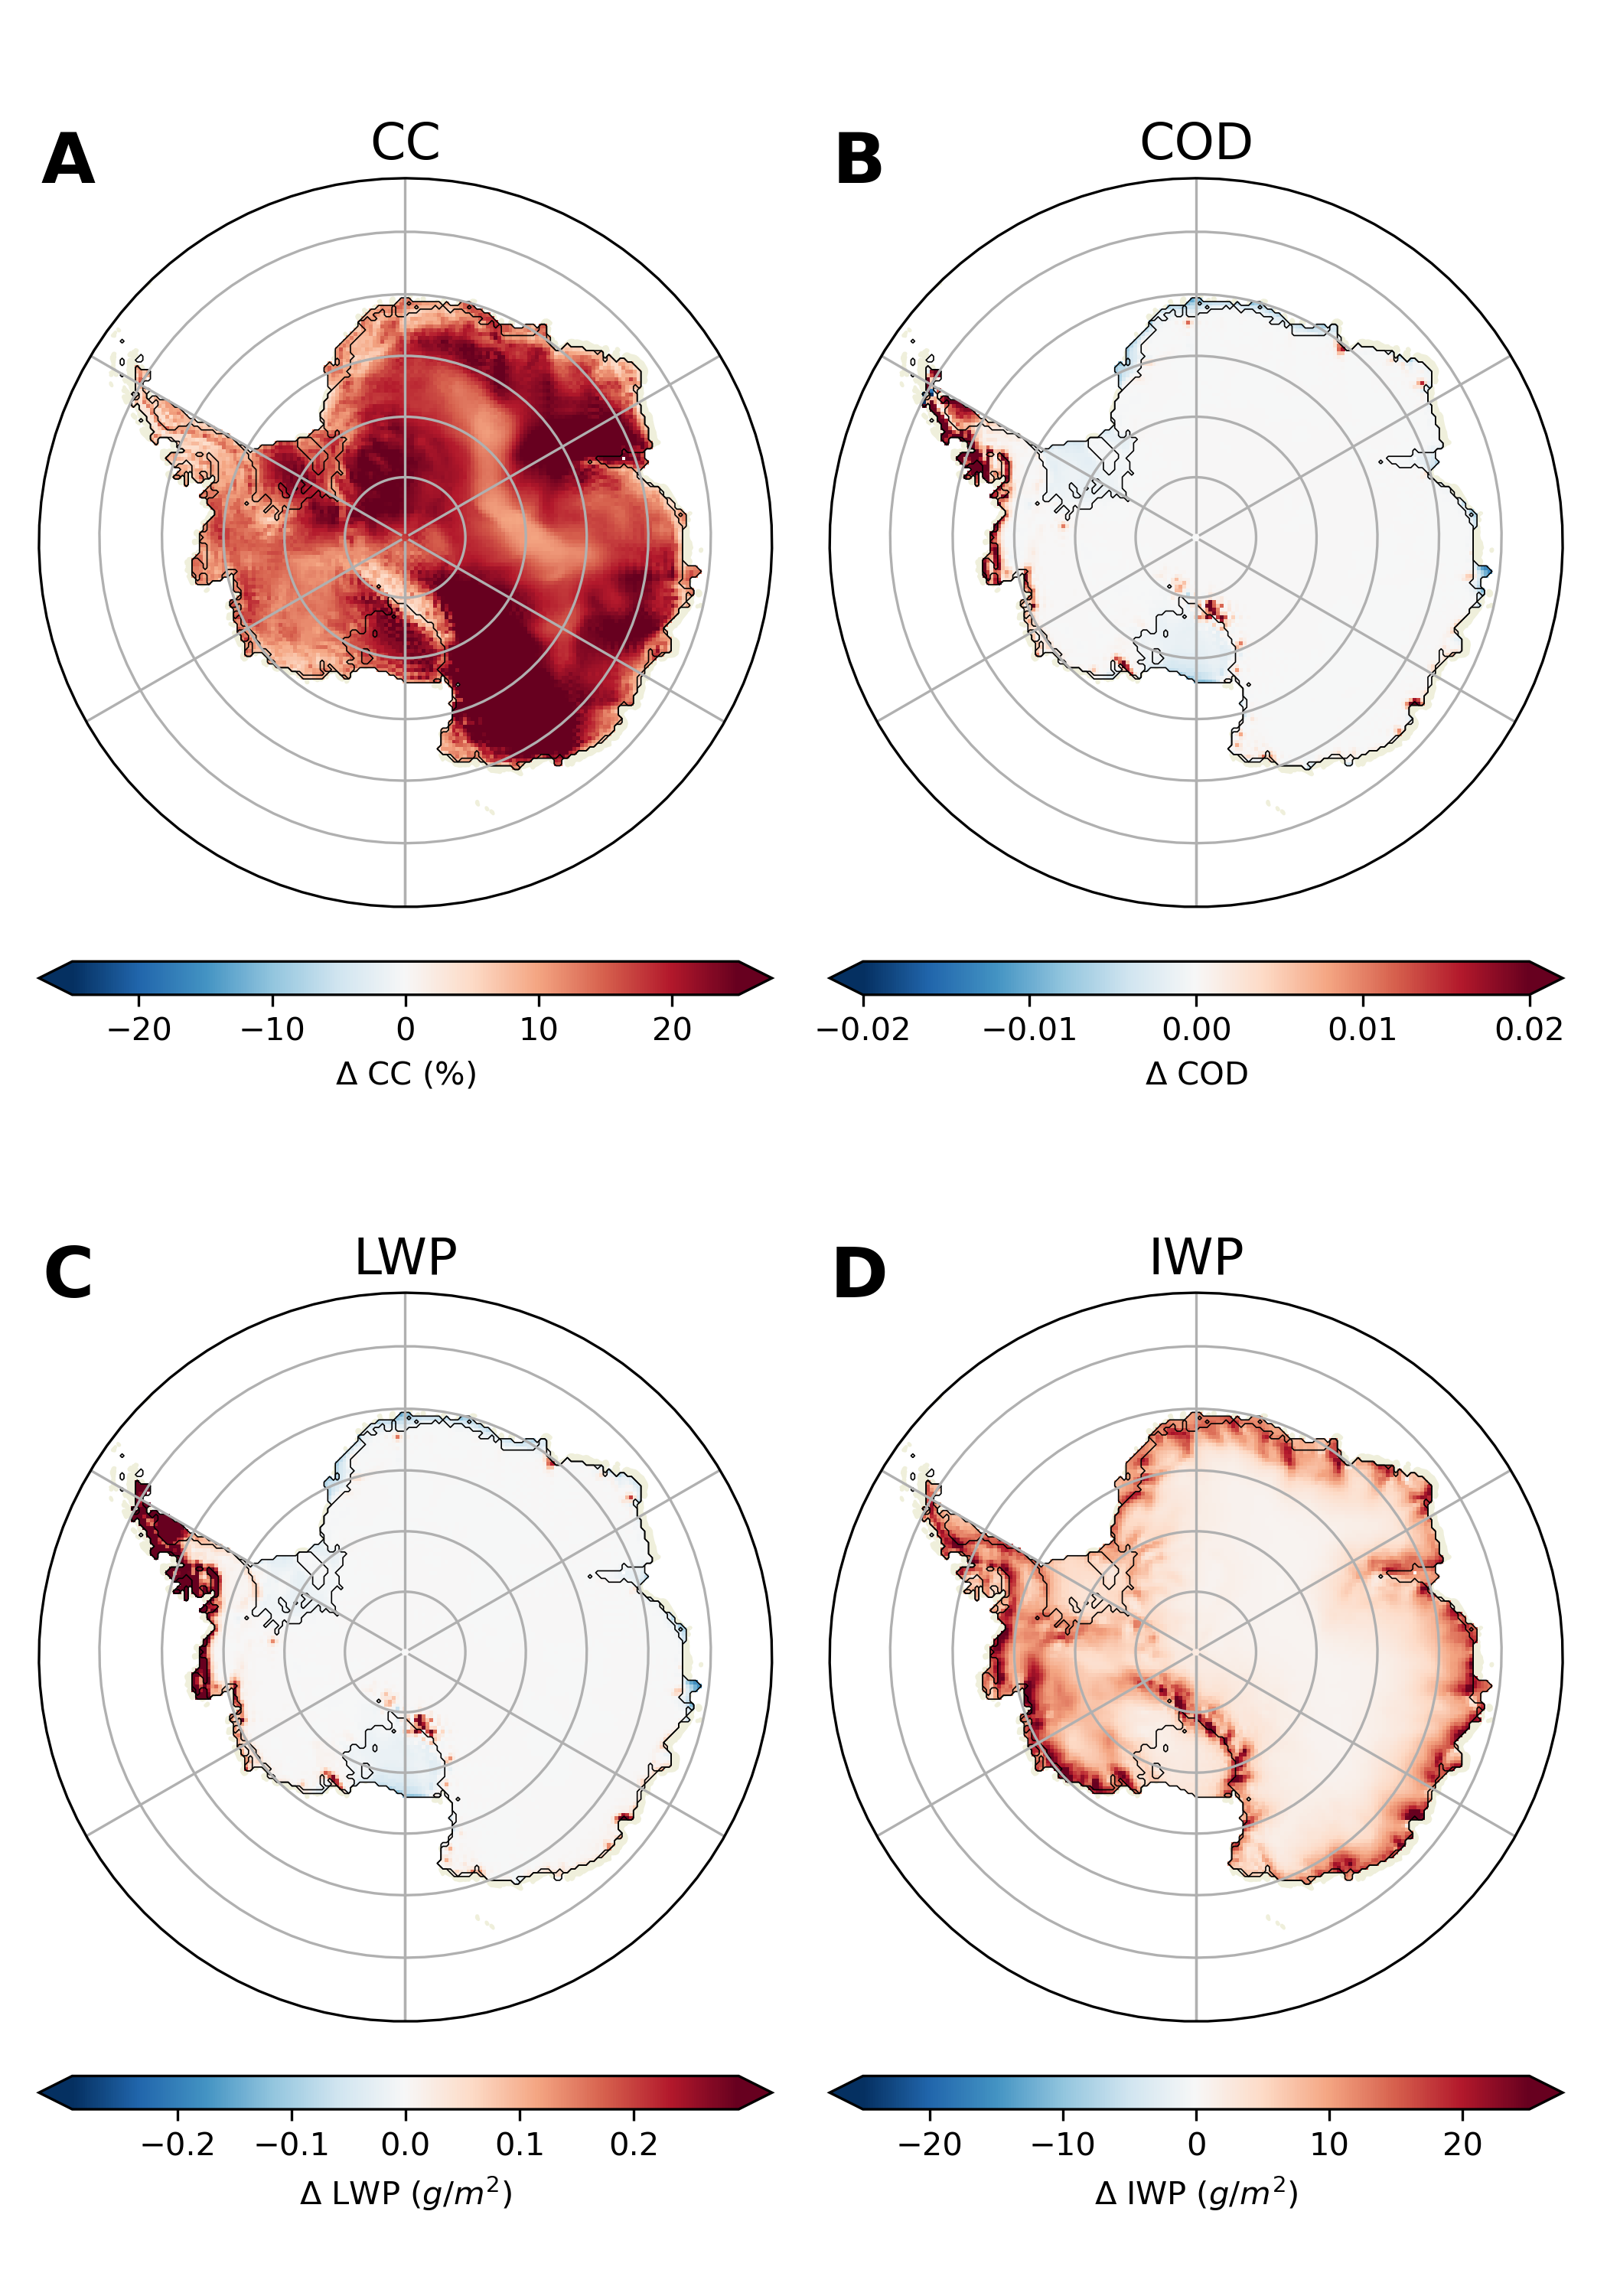
\includegraphics[scale=0.7]{microphysics.png}
	\caption{\textbf{Difference in cloud properties between MAR with and without drifting snow.} A) Difference in cloud cover (\%) between the two MAR simulations. Red colors indicate a greater cloud cover percentage in MAR with active drifting snow parameterisation. B) Same as A) but for the difference in cloud optical depth (COD, unitless) between the two MAR simulations. C) Same as A) but for the difference in liquid water path (LWP, g/m$^2$). D) Same as A) but for the difference in ice water path (IWP, g/m$^2$).}
	\label{fig:micro}
\end{figure}
%The strongest decrease in COD over open ocean waters is mainly a result of a decrease in cloud liquid water path (LWP) (Fig.\ref{fig:micro}C), in addition to a decrease in IWP (Fig.\ref{fig:micro}D). This decrease in COD, CC, LWP and IWP over the open ocean could be due to a decrease in cloud lifetime because of extra ice crystal numbers due to drifting snow, potentially increasing the glaciation rate of clouds via the Wegener-Bergeron-Findeisen process (\cite{Storelvmo2015, Gallee1994}) and subsequent increase in precipitation efficiency upstream of the Southern Ocean.

 Conversely, over the drier and colder interior of Antarctica, we see virtually no changes in liquid water path despite a significant increase in cloud cover (Fig.\ref{fig:micro}A-C). However, our results suggest a widespread increase in cloud ice water path (Fig.\ref{fig:micro}D), with a mean increase over the grounded AIS of +5.9\,g/m\textsuperscript{-2} and even more over the ice shelves with an increase of +9.1\,g/m\textsuperscript{-2} in MAR with drifting snow. These changes in cloud ice water path correspond to a +10.3\% increase over the grounded ice and a 10.2\% increase over the ice shelves  %Additionally, new ice particles can also grow in MAR due to higher relative humidity of the advected air via the gas phase or via heterogeneous and homogeneous freezing \cite{Gallee1994}.
 Note however, that the MAR cloud microphysics scheme currently does not account for secondary ice production, where one single ice crystal can turn into multiple ice crystals via collision breakup, drop shattering and rime splintering \cite{Gallee1994, Storelvmo2015, Soti2020, Field2017}. However, especially rime splintering and drop shattering need liquid to be present and are most efficient in temperatures above what we observe over Antarctica \cite{Soti2020}. Therefore, we do not think that the missing drop shattering and rime splintering processes are a major source of uncertainty in our simulations, however, collision breakup in drifting-snow clouds could be an important missing multiplier of ice crystal number concentration in our simulations.

\subsection{Comparison of cloud cover to satellite observations}


To find out how adding active drifting snow to MAR changes the modelled cloud cover, we compare MAR and ERA5 to the Cloudsat-Calipso active satellite cloud cover product \cite{kay2009, marchand2008, mace2009} (Fig.\ref{fig:sat} A-C). Over the periods where Cloudsat-Calipso data is available (07/2006-02/2011), we find that MAR without active drifting snow overestimates cloud cover by 7.9 $\pm$ 9.2\,\% (Fig.\ref{fig:sat} A). The slight overestimation seems to be enhanced over East Antarctica. Furthermore, MAR with active drifting snow increases the overestimation of cloud cover to 25.4$\pm$ 12.4\,\% (Fig.\ref{fig:sat} B). Otherwise, MAR with drifting snow shows a spatially homogenous bias with little spatial variability. For a better understanding where MAR cloud cover biases rank compared to the widely used state-of-the-art reanalysis product ERA5 \cite{Hersbach2020}, we also compare ERA5 to the Cloudsat-Calipso cloud cover product. ERA5 shows a slightly larger overestimation of cloud cover (9.8 $\pm$ 14.5\,\%) than MAR without drifting snow, but 15.6\% less than MAR with drifting snow.

\begin{figure}[H]
	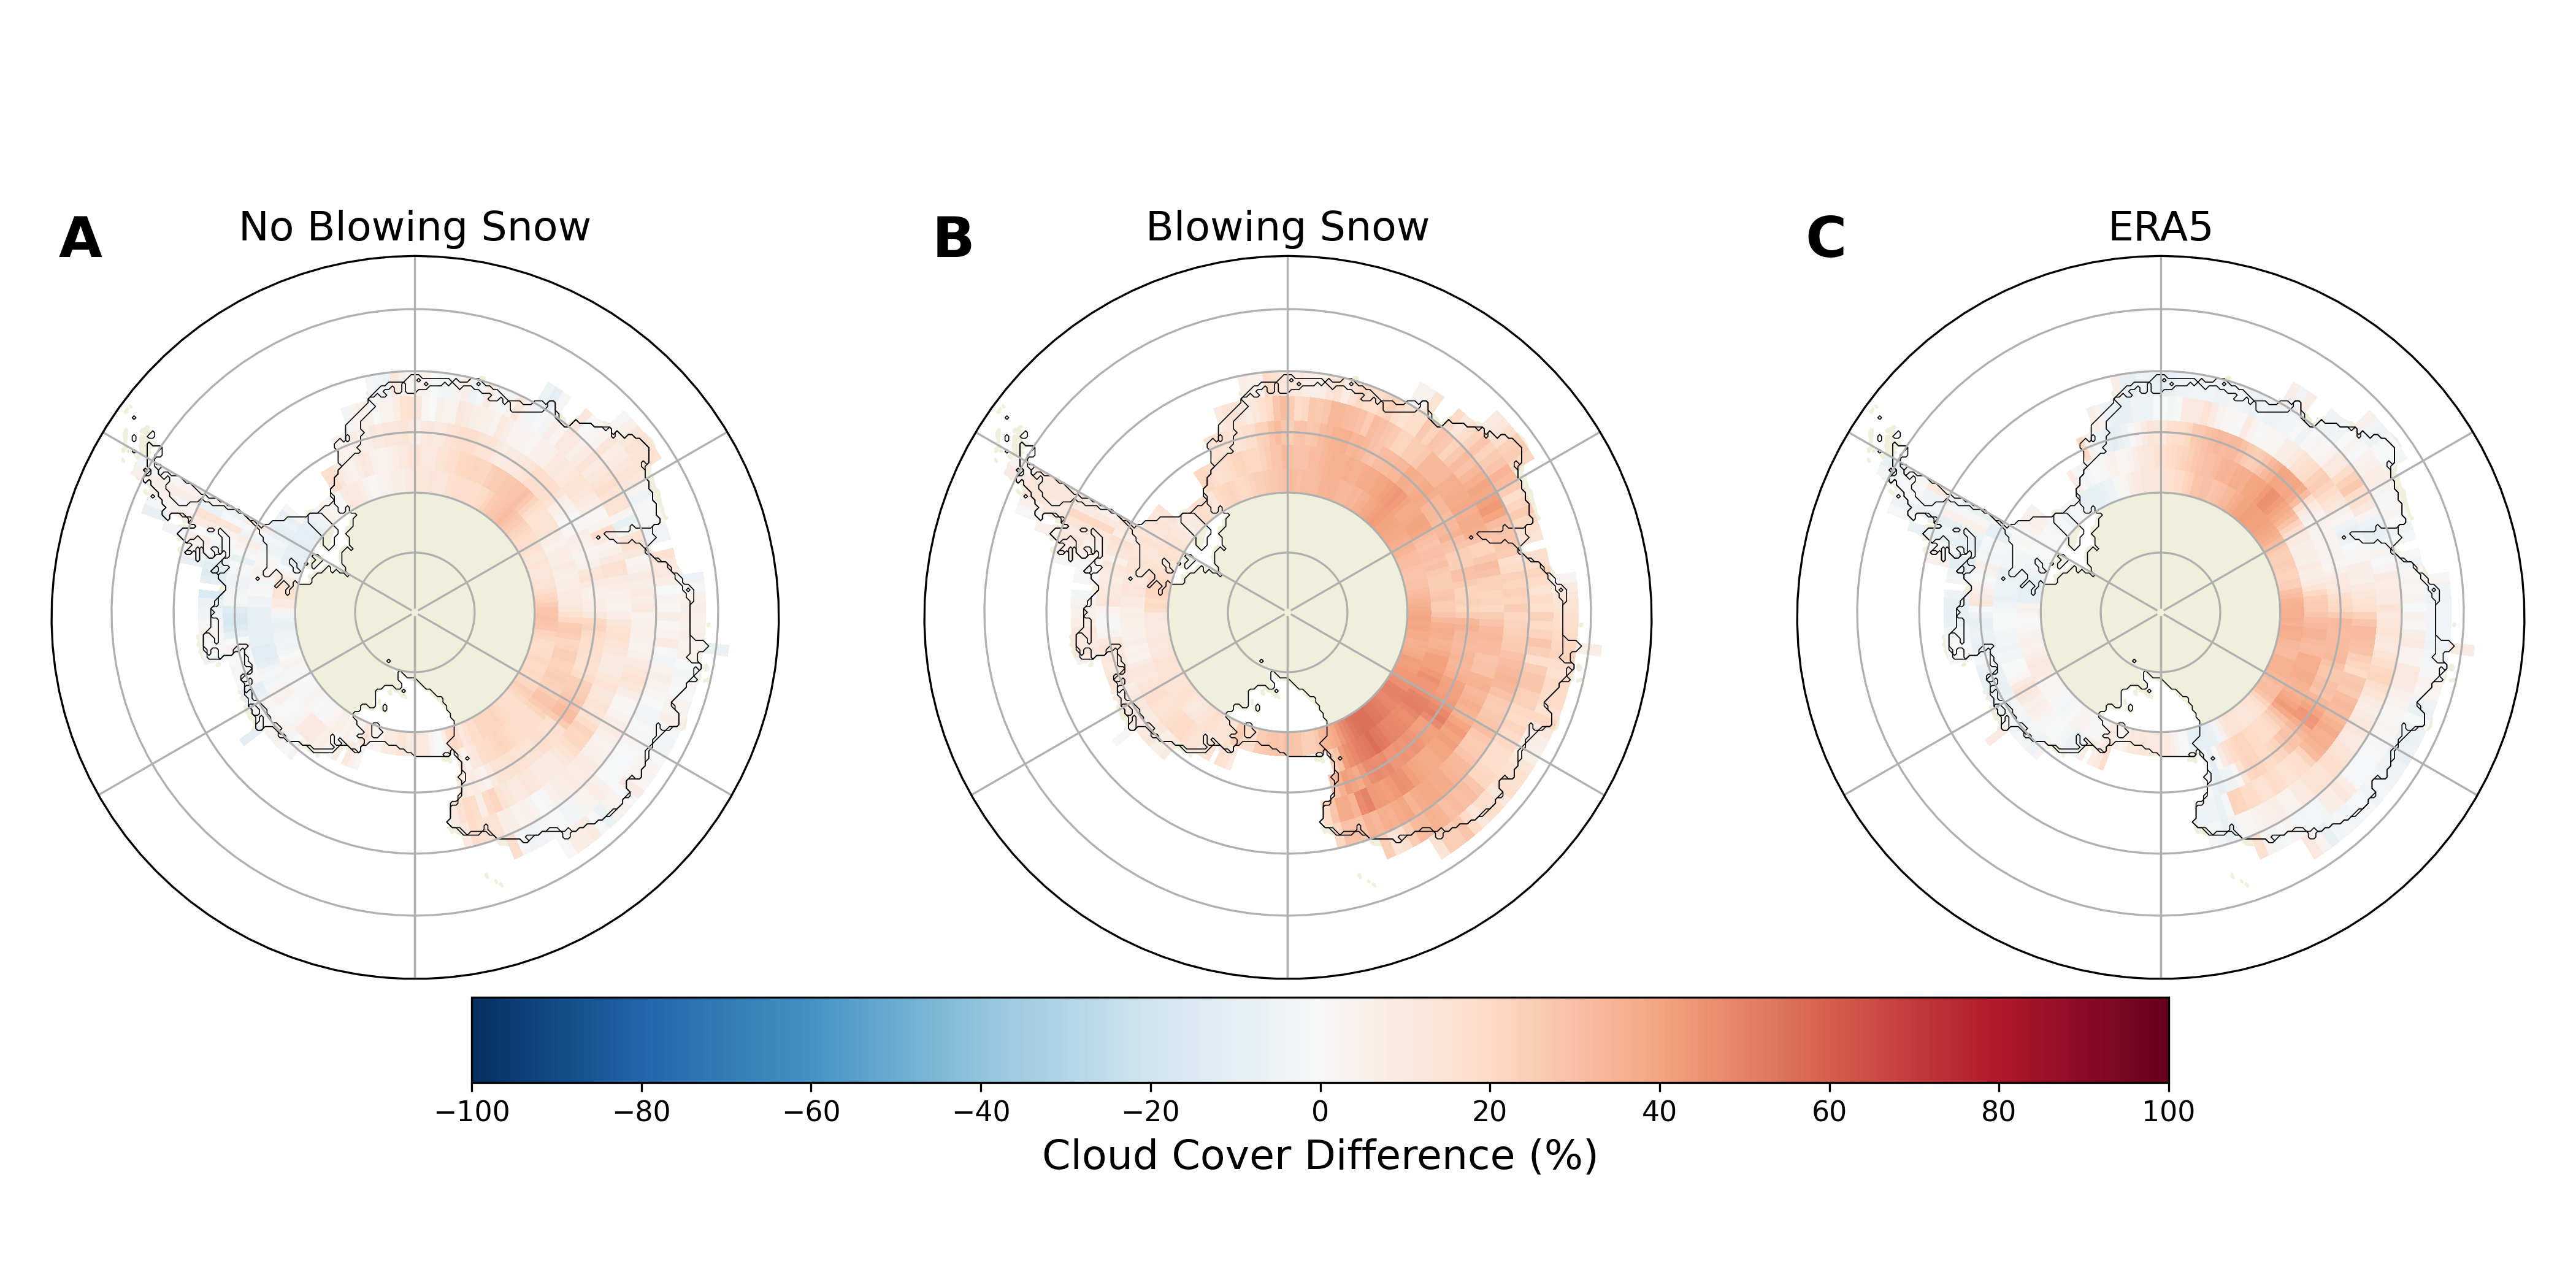
\includegraphics[width=1\textwidth]{Calipso_difference_new.png}
	\caption{\textbf{Comparison between Cloudsat-Calipso cloud cover, MAR and ERA5.} A) Comparison between MAR without drifting snow and Cloudsat-calipso cloud cover over 07/2006-02/2011. B) Same as A) but for the comparison with MAR including drifting snow. C) Comparison between ERA5 cloud cover and the Cloudsat-Calipso cloud cover.}
	\label{fig:sat}
\end{figure}

% CALIPSO COMPARISON VALUES
%NoBS mean: 7.93, NOBS STD: 9.24
%BS mean: 25.40, BS STD: 12.36
%ERA mean: 9.79, ERA STD: 14.45

Note however, that even though the global gridded CloudSat-CALIPSO cloud cover product here is one of the most advanced cloud products available for comparison with climate models, it does not include information about cloud cover below 720 m above the surface \cite{kay2009}. Therefore, because drifting-snow clouds are mostly less than 500 m in vertical extent \cite{Palm2018}, it is hard to assess with the currently available products whether accounting for drifting snow in MAR improves or degrades the performance with respect to cloud cover. Further, while there is only limited observational evidence for the size distribution of drifting snow particles, a case study over the South Pole station found that drifting snow particles are mostly between 30~{\textmu}m and 100~{\textmu}m in size \cite{Lawson2006}, a range also observed for typical cloud ice crystals. This similarity likely indicates that drifting snow clouds have similar optical and radiative properties to "conventional" clouds, and therefore information about drifting-snow clouds should be added to satellite cloud cover products over Antarctica.

\subsection{Influence of drifting snow on the Antarctic surface energy budget}

Changes in cloud macrophysical properties (cloud cover, ice and liquid water path) due to drifting snow go hand-in-hand with changes in the surface energy budget. In the shortwave part of the spectrum, our simulation with drifting snow shows less incoming solar radiation over Antarctica (Fig.\ref{fig:SEB}A), mostly due to an increase in cloud cover, and a slight increase in solid particle content as highlighted by IWP changes (Fig.\ref{fig:micro}A,D). On average, over the grounded Antarctica Ice Sheet the SWD decrease is -0.49\,Wm\textsuperscript{-2} and over the ice shelves it is -0.20\,Wm\textsuperscript{-2}. The second driver of the surface energy budget, downwelling longwave radiation, shows the opposite effect: LWD increases over all the grounded Antarctic Ice Sheet (+1.65\,Wm\textsuperscript{-2}) and over the ice shelves (+0.99\,Wm\textsuperscript{-2}) when drifting snow is active.

\begin{figure}[H]
	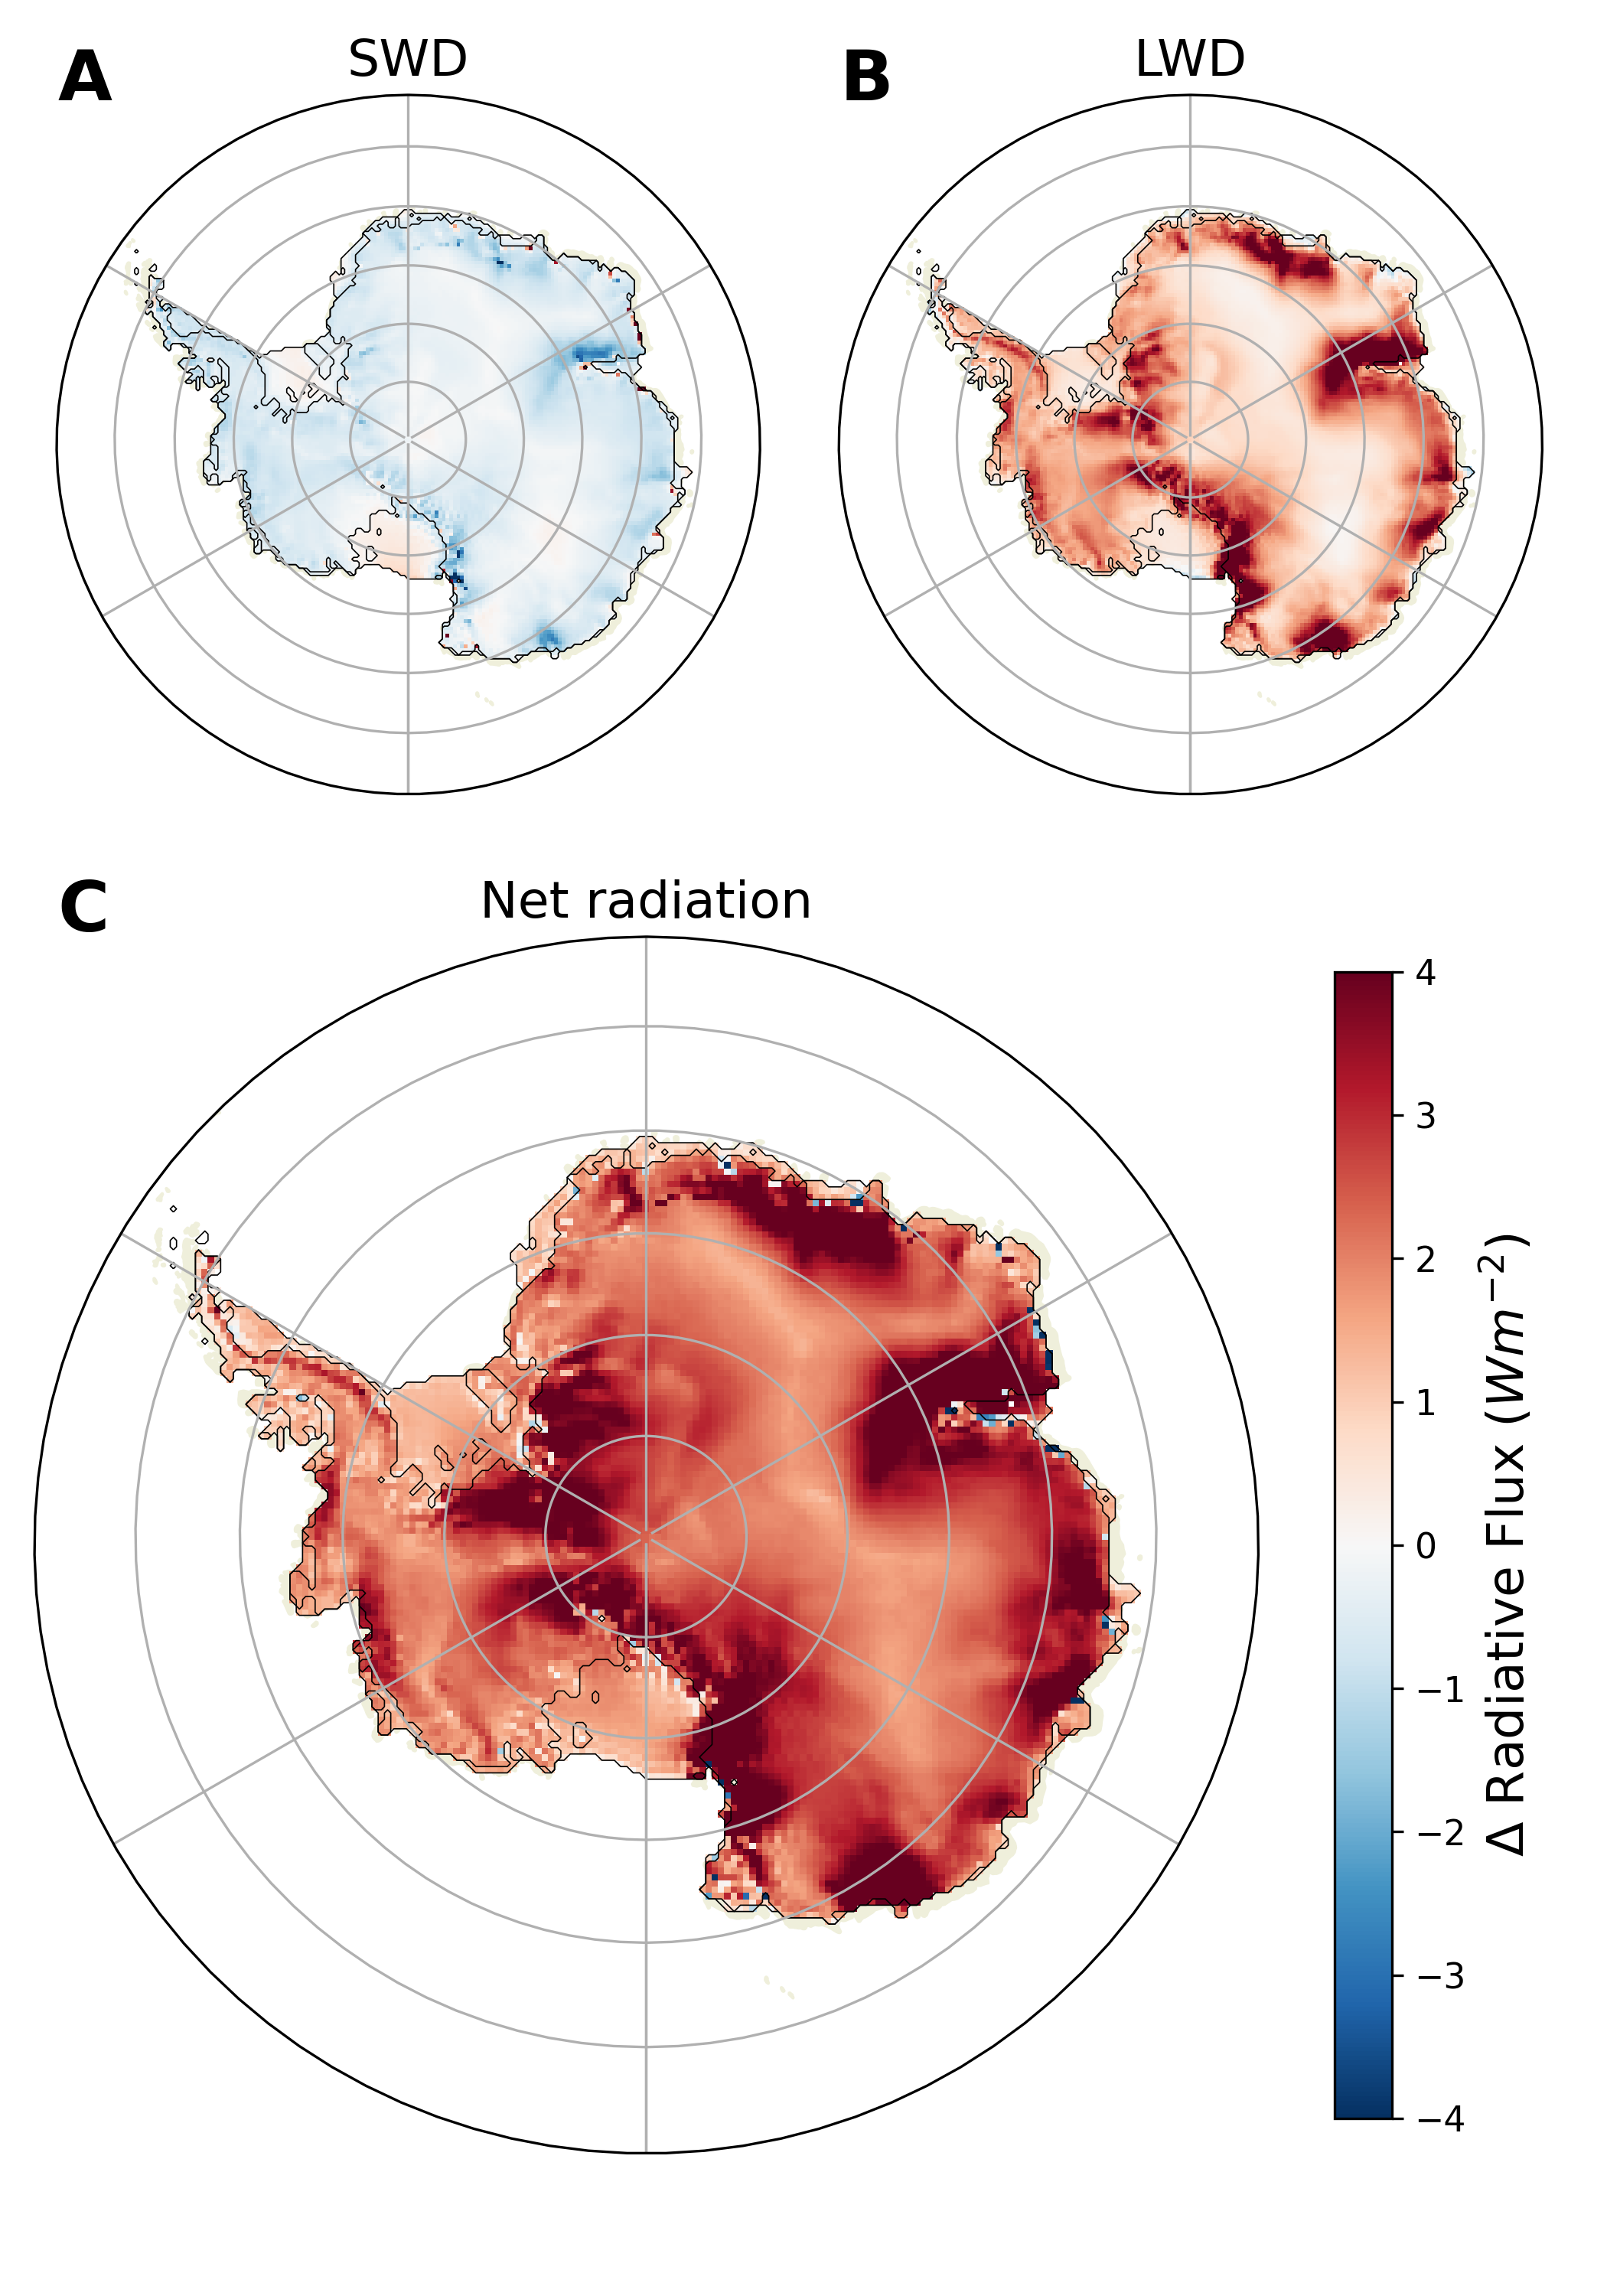
\includegraphics[scale=0.65]{SEB.png}
	\caption{\textbf{Difference in radiative components at the surface between MAR with and without drifting snow.} A) Difference in incoming shortwave radiation (SWD) at the surface in $Wm^{-2}$. Red color indicates a greater downwelling shortwave flux in MAR with active drifting snow parameterisation. B) Same A) but for the downwelling longwave flux at the surface. C) Same as A) and B), but for the difference in the net radiation at the surface ($R= SWD * (1 - \alpha) + LWD - LWU$).}
	\label{fig:SEB}
\end{figure}

%New values
%SWD: Grounded=-0.49, Shelves=-0.20, Ocean=nan
%LWD: Grounded=1.65, Shelves=0.99, Ocean=nan
%Net diff: Grounded=2.74, Shelves=1.43, Ocean=nan

When looking at the net radiative effect of drifting snow (Fig.\ref{fig:SEB}C), we see that including drifting snow leads to a net radiative warming of +2.74\,Wm\textsuperscript{-2} over the grounded Antarctic Ice Sheet and +1.43\,Wm\textsuperscript{-2} over the ice shelves. Here, the radiative warming effect is mostly caused by an increase in LWD, most notably over the steep margins, and by a decrease in outgoing longwave radiation due to sublimation of drifting-snow particles cooling the near surface atmosphere. We find only limited evidence for a notable contribution of net shortwave radiation through changes in the surface albedo when accounting for drifting snow (not shown). Over the steeper terrain we see an increase in cloud cover, together with the strongest increase in cloud ice water path due to greater wind speeds and snow erosion, causing an enhanced atmospheric longwave emissivity (Fig.\ref{fig:micro}D).

For future sea level rise projections, the most important result is that drifting snow can induce a radiative warming over Antarctica (Fig.\ref{fig:SEB}C). However, drifting snow is currently not implemented in many state-of-the-art climate models, and drifting-snow modelling approaches do not systematically account for explicit vertical advection of drifting-snow particles in the atmosphere, nor for their thermodynamic and radiative interactions with the atmosphere \cite{Lenaerts2012a}. Therefore, drifting snow represents a source of uncertainty for future projections of the Antarctic surface energy budget response to a warming climate, especially given that surface melt has been identified as an increasing surface ablation component over the ice shelves in Antarctic climate projections \cite{Kittel2021}.

\subsection{Comparison with in-situ weather station data}

When comparing MAR to 20 in-situ weather station observations across the Antarctic Ice Sheet, the mean bias is notably reduced in our simulation with active drifting snow (Fig. \ref{fig:heat}, the mean bias for individual stations can be found in Supplementary Fig.~1). The reduction of the mean bias in absolute terms is greatest in the longwave part of the spectrum with -1.1\,Wm\textsuperscript{-2} in the downwelling longwave radiation (LWD) and -1.6\,Wm\textsuperscript{-2} in the outgoing longwave radiation (LWU, Fig. \ref{fig:heat} first row). Additionally, MAR with drifting snow has no notable impact on the outgoing shortwave radiation (SWU), where the mean bias is almost constant at +0.07\,Wm\textsuperscript{-2}, while it is slightly increased in the downwelling shortwave component (SWD) at +0.46\,Wm\textsuperscript{-2}. Overall, acounting for drifting snow in MAR over Antarctica leads to a 2.17\,Wm\textsuperscript{-2} better representation of the radiative fluxes when compared to observations (-1.6 - 1.1 +0.07 + 0.46 = -2.17\,Wm\textsuperscript{-2}). The greatest improvement in the mean bias is related to the two longwave components of the surface energy budget when explicitly modelling drifting snow over Antarctica.


\begin{figure}[H]
	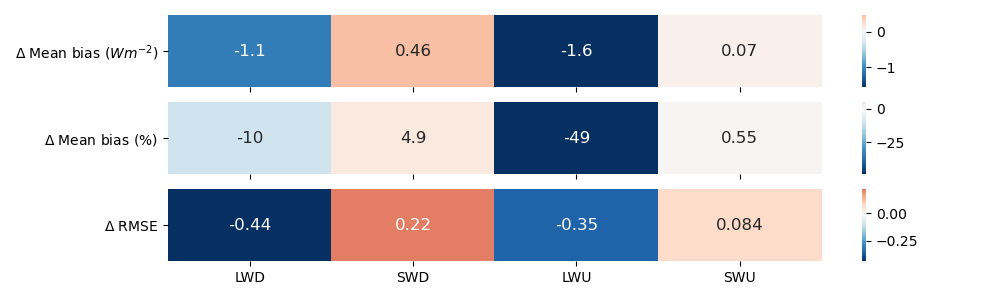
\includegraphics[width=1.1\textwidth]{heatmap_new.png}
	\caption{\textbf{Statistical comparison of MAR to 20 in-situ weather stations over Antarctica.} \textbf{First row:} change in the mean bias (Wm\textsuperscript{-2}) when comparing MAR with drifting snow to 20 in-situ observations over the entire Antarctic Ice Sheet in contrast to MAR without drifting snow. From left to right the numbers indicate the changes for incoming longwave (LWD), incoming shortwave (SWD), outgoing longwave (LWU) and outgoing (reflected) shortwave radiation (SWU). Negative numbers indicate a better comparison to the observations when drifting snow is activate in MAR. \textbf{Second row}: same as first row but for the percentage reduction/increase in the absolute value of the mean bias when comparing to MAR without drifting snow. \textbf{Third row:} same as first row but the change in the root-mean-square-error (RMSE).}
	\label{fig:heat}
\end{figure}

Comparing the change in the mean biases when accounting for drifting snow in MAR to the initial absolute mean biases of the control simulation without drifting snow we see a slightly different weighting (Fig. \ref{fig:heat}, second row). Our model results with drifting snow show a -49.0\% decrease of the mean bias in LWU, followed by a -10.0\% decrease in the LWD mean bias. Slightly less pronounced are the changes in SWU at +0.55\% and a slight increase of 4.9\% in the SWD component (Fig. \ref{fig:heat}, second row). Conversely, the largest improvement in the root-mean-square-error (RMSE) occurs in LWD (-0.44\,Wm\textsuperscript{-2}, Fig. \ref{fig:heat},third row) and LWU (-0.35\,Wm\textsuperscript{-2}).  Additionally, accounting for drifting snow leads to a minor increase in the RMSE in SWU of +0.084 and a slightly higher RMSE in the SWD component of +0.22\,Wm\textsuperscript{-2}. Overall, we again see the most notable improvement when using the active drifting snow scheme in MAR is in the incoming and outgoing longwave radiation.

\section*{Discussion}

Actively modelling drifting snow in a state-of-the-art polar regional climate model (MAR) sheds light on the complex interactions between drifting-snow particles, clouds and subsequently the Antarctic surface energy budget. Our simulation with drifting snow clearly differ from our control simulation in 3 different ways:
1) Drifting-snow particles change the micro- and macrophysical properties of clouds by acting as a radiatively active cloud themselves, enhancing the moisture availability due to sublimation, and also potentially as cloud nuclei enhancing the Wegener-Bergeron-Findeisen process.
2) Drifting-snow particles change the structure of the near-surface atmosphere, mainly by inducing sublimation cooling and by providing a notable source of moisture.
3) Drifting snow alters the cloud radiative effect and increases cloud cover across Antarctica, enhancing the atmospheric longwave emissivity ($\epsilon$) and reducing the shortwave transmissivity of the atmosphere. 
Overall, modelling drifting snow over the Antarctic Ice Sheet notably changes the cloud structure and therefore the surface energy budget.

Our results also answer the question whether accounting for drifting snow leads to a net positive or negative radiative effect over Antarctica. We find that drifting snow leads to a net radiation increase at the surface of +2.74\,Wm\textsuperscript{-2} over the grounded parts of the Antarctic Ice Sheet, which could ultimately contribute to global sea level rise (Fig. \ref{fig:SEB}). Note however, that more local analysis suggests that a decrease in the latent heat flux through sublimation cooling might partly offset some of the radiative warming \cite{Letoumelin2020}.

Additionally, accounting for airborne snow particles also leads to a more accurate representation of the surface radiative energy budget when compared to 20 in-situ weather station observations. Overall, MAR with active drifting snow has a 2.17\,Wm\textsuperscript{-2} lower bias in radiative fluxes compared to the base version of MAR (Fig. \ref{fig:heat}). Most improved is the representation of the longwave components, almost halving the bias in outgoing longwave radiation (-49\%, -1.6\,Wm\textsuperscript{-2}), but also notably reducing the bias in downwelling longwave radiation (-10.0\%, -1.1\,Wm\textsuperscript{-2}) when compared to observations (Fig. \ref{fig:heat}).

Our results indicate that accounting for drifting snow is an important mechanism when modelling the current and future state of the Antarctic Ice Sheet. The additional radiation at the surface of +2.74 Wm\textsuperscript{-2} due to drifting snow in MAR is of similar or greater magnitude than the roughly +2.0\,Wm\textsuperscript{-2} that the Earth receives due to anthropogenic greenhouse gas emissions. Conversely, most of this radiative warming in our simulations occurs in the very cold interior plateau of Antarctica, where the surface temperatures are far below the melting point and the surface almost never melts. However, our results also show that essential cloud parameters are also altered over the margins and ice shelves, potentially indicating that future sea level rise projections need to take into account drifting snow as a key mechanism for accurate future Antarctic climate projections.
%%

%  Numbered lines in equations:
%  To add line numbers to lines in equations,
%  \begin{linenomath*}
%  \begin{equation}
%  \end{equation}
%  \end{linenomath*}



%% Enter Figures and Tables near as possible to where they are first mentioned:
%
% DO NOT USE \psfrag or \subfigure commands.
%
% Figure captions go below the figure.
% Table titles go above tables;  other caption information
%  should be placed in last line of the table, using
% \multicolumn2l{$^a$ This is a table note.}
%
%----------------
% EXAMPLE FIGURES
%
% \begin{figure}
% \includegraphics{example.png}
% \caption{caption}
% \end{figure}
%
% Giving latex a width will help it to scale the figure properly. A simple trick is to use \textwidth. Try this if large figures run off the side of the page.
% \begin{figure}
% \noindent\includegraphics[width=\textwidth]{anothersample.png}
%\caption{caption}
%\label{pngfiguresample}
%\end{figure}
%
%
% If you get an error about an unknown bounding box, try specifying the width and height of the figure with the natwidth and natheight options. This is common when trying to add a PDF figure without pdflatex.
% \begin{figure}
% \noindent\includegraphics[natwidth=800px,natheight=600px]{samplefigure.pdf}
%\caption{caption}
%\label{pdffiguresample}
%\end{figure}
%
%
% PDFLatex does not seem to be able to process EPS figures. You may want to try the epstopdf package.
%

%
% ---------------
% EXAMPLE TABLE
%
% \begin{table}
% \caption{Time of the Transition Between Phase 1 and Phase 2$^{a}$}
% \centering
% \begin{tabular}{l c}
% \hline
%  Run  & Time (min)  \\
% \hline
%   $l1$  & 260   \\
%   $l2$  & 300   \\
%   $l3$  & 340   \\
%   $h1$  & 270   \\
%   $h2$  & 250   \\
%   $h3$  & 380   \\
%   $r1$  & 370   \\
%   $r2$  & 390   \\
% \hline
% \multicolumn{2}{l}{$^{a}$Footnote text here.}
% \end{tabular}
% \end{table}

%% SIDEWAYS FIGURE and TABLE
% AGU prefers the use of {sidewaystable} over {landscapetable} as it causes fewer problems.
%
% \begin{sidewaysfigure}
% \includegraphics[width=20pc]{figsamp}
% \caption{caption here}
% \label{newfig}
% \end{sidewaysfigure}
%
%  \begin{sidewaystable}
%  \caption{Caption here}
% \label{tab:signif_gap_clos}
%  \begin{tabular}{ccc}
% one&two&three\\
% four&five&six
%  \end{tabular}
%  \end{sidewaystable}

%% If using numbered lines, please surround equations with \begin{linenomath*}...\end{linenomath*}
%\begin{linenomath*}
%\begin{equation}
%y|{f} \sim g(m, \sigma),
%\end{equation}
%\end{linenomath*}

%%% End of body of article

%%%%%%%%%%%%%%%%%%%%%%%%%%%%%%%%
%% Optional Appendix goes here
%
% The \appendix command resets counters and redefines section heads
%
% After typing \appendix
%
%\section{Here Is Appendix Title}
% will show
% A: Here Is Appendix Title
%
%\appendix
%\section{Here is a sample appendix}

%%%%%%%%%%%%%%%%%%%%%%%%%%%%%%%%%%%%%%%%%%%%%%%%%%%%%%%%%%%%%%%%
%
% Optional Glossary, Notation or Acronym section goes here:
%
%%%%%%%%%%%%%%
% Glossary is only allowed in Reviews of Geophysics
%  \begin{glossary}
%  \term{Term}
%   Term Definition here
%  \term{Term}
%   Term Definition here
%  \term{Term}
%   Term Definition here
%  \end{glossary}

%
%%%%%%%%%%%%%%
% Acronyms
%   \begin{acronyms}
%   \acro{Acronym}
%   Definition here
%   \acro{EMOS}
%   Ensemble model output statistics
%   \acro{ECMWF}
%   Centre for Medium-Range Weather Forecasts
%   \end{acronyms}

%
%%%%%%%%%%%%%%
% Notation
%   \begin{notation}
%   \notation{$a+b$} Notation Definition here
%   \notation{$e=mc^2$}
%   Equation in German-born physicist Albert Einstein's theory of special
%  relativity that showed that the increased relativistic mass ($m$) of a
%  body comes from the energy of motion of the body—that is, its kinetic
%  energy ($E$)—divided by the speed of light squared ($c^2$).
%   \end{notation}




%%%%%%%%%%%%%%%%%%%%%%%%%%%%%%%%%%%%%%%%%%%%%%%%%%%%%%%%%%%%%%%%
%
%  ACKNOWLEDGMENTS
%
% The acknowledgments must list:
%
% >>>>	A statement that indicates to the reader where the data
% 	supporting the conclusions can be obtained (for example, in the
% 	references, tables, supporting information, and other databases).
%
% 	All funding sources related to this work from all authors
%
% 	Any real or perceived financial conflicts of interests for any
%	author
%
% 	Other affiliations for any author that may be perceived as
% 	having a conflict of interest with respect to the results of this
% 	paper.
%
%
% It is also the appropriate place to thank colleagues and other contributors.
% AGU does not normally allow dedications.


\acknowledgments
This project has received funding from the European Research Council (ERC) under the European Union’s Horizon 2020 research and innovation programme (Grant agreement No. 758005).

\subsubsection*{Author contributions}

S.H., C.A., C.K., T.S., L.L, and T.C designed the study. C.A. and C.K. developed the model configuration and performed the simulations. S.H., C.K and C.A. analyzed the data, T.C provided the satellite data. S.H. wrote the manuscript. All authors discussed the final version of manuscript.

\subsubsection*{Competing interests}
The authors declare that they have no competing interests.

\subsubsection*{Code and data availability}

%The monthly means used in this study, from 1980-2100 of all three MAR RCP 8.5 simulations are available via ftp://ftp.climato.be/fettweis/MARv3.9/Greenland/. In case daily outputs are required, these can be requested from Xavier Fettweis (xavier.fettweis@uliege.be) and Stefan Hofer (s.hofer@bristol.ac.uk).
%
\textbf{Data and code owned by the authors:} all the code used for the analysis in this study is available on https://github.com/stefan-hofer/Antarctica\_clouds, but will be made available via zenodo upon acceptance of the manuscript. All the 2000-2019 averages from our MAR simulations with and without blowing snow are available via \hfill \break  https://zenodo.org/record/5037197. 


\textbf{Data not owned by the authors:} We retrieved the "The Climate Data Guide: Combined CloudSat spaceborne radar and CALIPSO spaceborne lidar cloud fraction dataset" (last modified 21 April 2014) from https://climatedataguide.ucar.edu/climate-data/combined-cloudsat-spaceborne-radar-and-calipso-spaceborne-lidar-cloud-fraction-dataset and gratefully acknowledge Jennifer Kay and the National Center for Atmospheric Research Staff (Eds). The ERA5 data is available via the COPERNICUS Climate Data Store \hfill \break 
(https://cds.climate.copernicus.eu/\#!/home).

The weather station data used for comparison with MAR is a compilation of various sources.\hfill \break 
\textbf{D17:} https://zenodo.org/record/4139737 \hfill \break 
\textbf{Dome\_C\_II:} freely downloaded from the BSRN website: https://bsrn.awi.de/ \hfill \break 
\textbf{Halley:} BSNR \hfill \break 
\textbf{Amundsen\_Scott:} BSRN \hfill \break 
\textbf{Neumayer, Sorasen et Panda-1:} contact Holger Schmithuesen: holger.schmithuesen@awi.de (AWI) \hfill \break 
\textbf{From AWS4 to AWS19:} contact Constantijn L. Jakobs C.L.Jakobs@uu.nl (IMAU) \hfill \break 

%% ------------------------------------------------------------------------ %%
%% References and Citations

%%%%%%%%%%%%%%%%%%%%%%%%%%%%%%%%%%%%%%%%%%%%%%%
%
%\bibliography{<name of your .bib file>} don't specify the file extension
%
% don't specify bibliographystyle
%%%%%%%%%%%%%%%%%%%%%%%%%%%%%%%%%%%%%%%%%%%%%%%

\bibliography{agusample}



%Reference citation instructions and examples:
%
% Please use ONLY \cite and \citeA for reference citations.
% \cite for parenthetical references
% ...as shown in recent studies (Simpson et al., 2019)
% \citeA for in-text citations
% ...Simpson et al. (2019) have shown...
%
%
%...as shown by \citeA{jskilby}.
%...as shown by \citeA{lewin76}, \citeA{carson86}, \citeA{bartoldy02}, and \citeA{rinaldi03}.
%...has been shown \cite{jskilbye}.
%...has been shown \cite{lewin76,carson86,bartoldy02,rinaldi03}.
%... \cite <i.e.>[]{lewin76,carson86,bartoldy02,rinaldi03}.
%...has been shown by \cite <e.g.,>[and others]{lewin76}.
%
% apacite uses < > for prenotes and [ ] for postnotes
% DO NOT use other cite commands (e.g., \citet, \citep, \citeyear, \nocite, \citealp, etc.).
%



\end{document}



More Information and Advice:

%% ------------------------------------------------------------------------ %%
%
%  SECTION HEADS
%
%% ------------------------------------------------------------------------ %%

% Capitalize the first letter of each word (except for
% prepositions, conjunctions, and articles that are
% three or fewer letters).

% AGU follows standard outline style; therefore, there cannot be a section 1 without
% a section 2, or a section 2.3.1 without a section 2.3.2.
% Please make sure your section numbers are balanced.
% ---------------
% Level 1 head
%
% Use the \section{} command to identify level 1 heads;
% type the appropriate head wording between the curly
% brackets, as shown below.
%
%An example:
%\section{Level 1 Head: Introduction}
%
% ---------------
% Level 2 head
%
% Use the \subsection{} command to identify level 2 heads.
%An example:
%\subsection{Level 2 Head}
%
% ---------------
% Level 3 head
%
% Use the \subsubsection{} command to identify level 3 heads
%An example:
%\subsubsection{Level 3 Head}
%
%---------------
% Level 4 head
%
% Use the \subsubsubsection{} command to identify level 3 heads
% An example:
%\subsubsubsection{Level 4 Head} An example.
%
%% ------------------------------------------------------------------------ %%
%
%  IN-TEXT LISTS
%
%% ------------------------------------------------------------------------ %%
%
% Do not use bulleted lists; enumerated lists are okay.
% \begin{enumerate}
% \item
% \item
% \item
% \end{enumerate}
%
%% ------------------------------------------------------------------------ %%
%
%  EQUATIONS
%
%% ------------------------------------------------------------------------ %%

% Single-line equations are centered.
% Equation arrays will appear left-aligned.

Math coded inside display math mode \[ ...\]
 will not be numbered, e.g.,:
 \[ x^2=y^2 + z^2\]

 Math coded inside \begin{equation} and \end{equation} will
 be automatically numbered, e.g.,:
 \begin{equation}
 x^2=y^2 + z^2
 \end{equation}


% To create multiline equations, use the
% \begin{eqnarray} and \end{eqnarray} environment
% as demonstrated below.
\begin{eqnarray}
  x_{1} & = & (x - x_{0}) \cos \Theta \nonumber \\
        && + (y - y_{0}) \sin \Theta  \nonumber \\
  y_{1} & = & -(x - x_{0}) \sin \Theta \nonumber \\
        && + (y - y_{0}) \cos \Theta.
\end{eqnarray}

%If you don't want an equation number, use the star form:
%\begin{eqnarray*}...\end{eqnarray*}

% Break each line at a sign of operation
% (+, -, etc.) if possible, with the sign of operation
% on the new line.

% Indent second and subsequent lines to align with
% the first character following the equal sign on the
% first line.

% Use an \hspace{} command to insert horizontal space
% into your equation if necessary. Place an appropriate
% unit of measure between the curly braces, e.g.
% \hspace{1in}; you may have to experiment to achieve
% the correct amount of space.


%% ------------------------------------------------------------------------ %%
%
%  EQUATION NUMBERING: COUNTER
%
%% ------------------------------------------------------------------------ %%

% You may change equation numbering by resetting
% the equation counter or by explicitly numbering
% an equation.

% To explicitly number an equation, type \eqnum{}
% (with the desired number between the brackets)
% after the \begin{equation} or \begin{eqnarray}
% command.  The \eqnum{} command will affect only
% the equation it appears with; LaTeX will number
% any equations appearing later in the manuscript
% according to the equation counter.
%

% If you have a multiline equation that needs only
% one equation number, use a \nonumber command in
% front of the double backslashes (\\) as shown in
% the multiline equation above.

% If you are using line numbers, remember to surround
% equations with \begin{linenomath*}...\end{linenomath*}

%  To add line numbers to lines in equations:
%  \begin{linenomath*}
%  \begin{equation}
%  \end{equation}
%  \end{linenomath*}



